\documentclass[tikz]{standalone}

\begin{document}
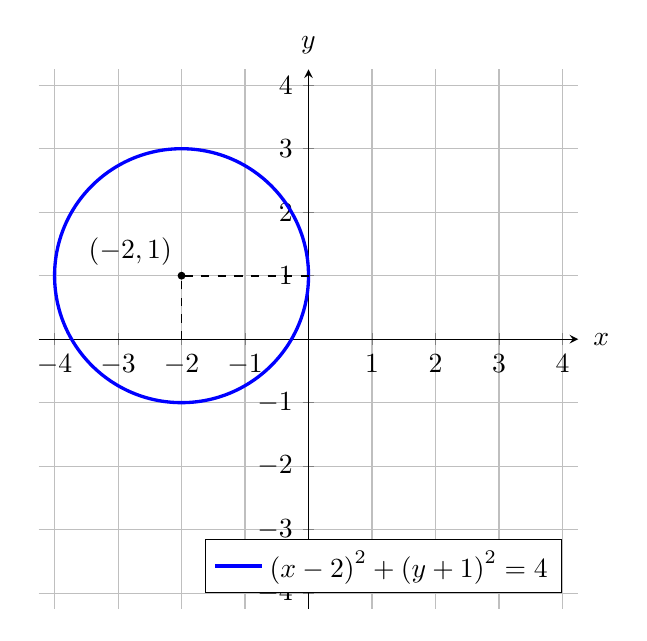
\begin{tikzpicture}
    \begin{axis}[%
        xlabel=$x$, ylabel=$y$, legend pos=south east,
        grid=both, axis lines = middle,
        minor x tick num=1, minor y tick num=1,
        xlabel style = {at={(axis description cs:1.01,0.5)},anchor=west},
        ylabel style = {at={(axis description cs:0.5,1.01)},anchor=south},
        xmin=-4.25, xmax=4.25, ymin=-4.25, ymax=4.25,
        xtick = {-4,-3,-2,-1,1,2,3,4}, ytick = {-4,-3,-2,-1,1,2,3,4},
        width=\axisdefaultwidth, height=\axisdefaultwidth,
    ]
    \addplot[very thick, blue] (-2,1) circle [radius=2];
    \fill[black] (-2,1) circle (.5mm) node[above left]{$(-2,1)$};
    \draw[semithick, dashed] (-2,0) |- (0,1);
    \legend{\({(x-2)}^2+{(y+1)}^2=4\)}
    \end{axis}
\end{tikzpicture}
\end{document}
